\documentclass{article}
\usepackage{amsmath}
\usepackage{graphicx}
\usepackage[margin=1in]{geometry}

\title{ML-Assisted Avalanche Effect Analyzer for AES}
\author{}
\date{}

\begin{document}

\maketitle

\section{Objective}

To analyze the avalanche effect in the Advanced Encryption Standard (AES) and apply machine learning techniques to study how small changes in plaintext influence ciphertext diffusion.

\section{Introduction}

AES is a widely used symmetric block cipher that operates on 128-bit blocks of data. One of the important security properties of AES is the avalanche effect. 

The avalanche effect means that a small change in the input, such as flipping a single bit in the plaintext, should cause a significant change in the output ciphertext. Ideally, about half of the ciphertext bits should change.

This property ensures strong diffusion and prevents attackers from predicting how input changes affect the encrypted output.

\section{AES Overview}

AES encryption consists of multiple rounds of transformations including:

\begin{itemize}
\item SubBytes
\item ShiftRows
\item MixColumns
\item AddRoundKey
\end{itemize}

These operations together provide confusion and diffusion in the encryption process.

\section{Methodology}

We implemented an experiment to study the avalanche effect in AES.

The steps followed were:

\begin{enumerate}
\item Generate random 128-bit plaintext
\item Flip a single bit in the plaintext (the bit was flipped using a bitwise XOR operation, creating a second plaintext that differs from the original exactly by one bit).
\item Encrypt both plaintexts using AES
\item Compare the resulting ciphertexts
\item Count the number of differing bits
\item Compute avalanche score = changed bits / 128
\end{enumerate}

We repeated this experiment for 2000 samples to build a dataset.

\section{Machine Learning Analysis}

We applied machine learning models to analyze whether the bit position flipped in the plaintext could predict the avalanche score.

The models used were:

\begin{itemize}
\item Linear Regression
\item Polynomial Regression
\item Random Forest
\end{itemize}

The dataset was split into training, validation, and test sets.

\section{Results}

The avalanche score is defined as the ratio of the number of differing ciphertext bits to the total number of bits in the AES block:

\[
\text{Avalanche Score} = \frac{\text{Number of differing ciphertext bits}}{128}
\]

AES operates on 128-bit blocks. For a secure cipher exhibiting the avalanche property, flipping a single input bit should cause each output bit to change with approximately 50\% probability. Statistically, this means that about half of the ciphertext bits (approximately 64 out of 128 bits) should change on average.

\[
\frac{64}{128} = 0.5
\]

In our experiment, the average avalanche value observed was:

\[
0.5014 \approx 0.5
\]

which closely matches the theoretical expectation for a secure cipher.

To further analyze the behavior, machine learning models were trained to predict the avalanche score using the flipped bit position as the input feature. All models produced $R^2$ values close to zero or negative. This indicates that the bit position carries little or no predictive information about the avalanche score.

This result confirms that diffusion in AES is uniform across all input bits, meaning that the ciphertext changes are essentially independent of which plaintext bit was flipped.

\begin{figure}[h]
\centering
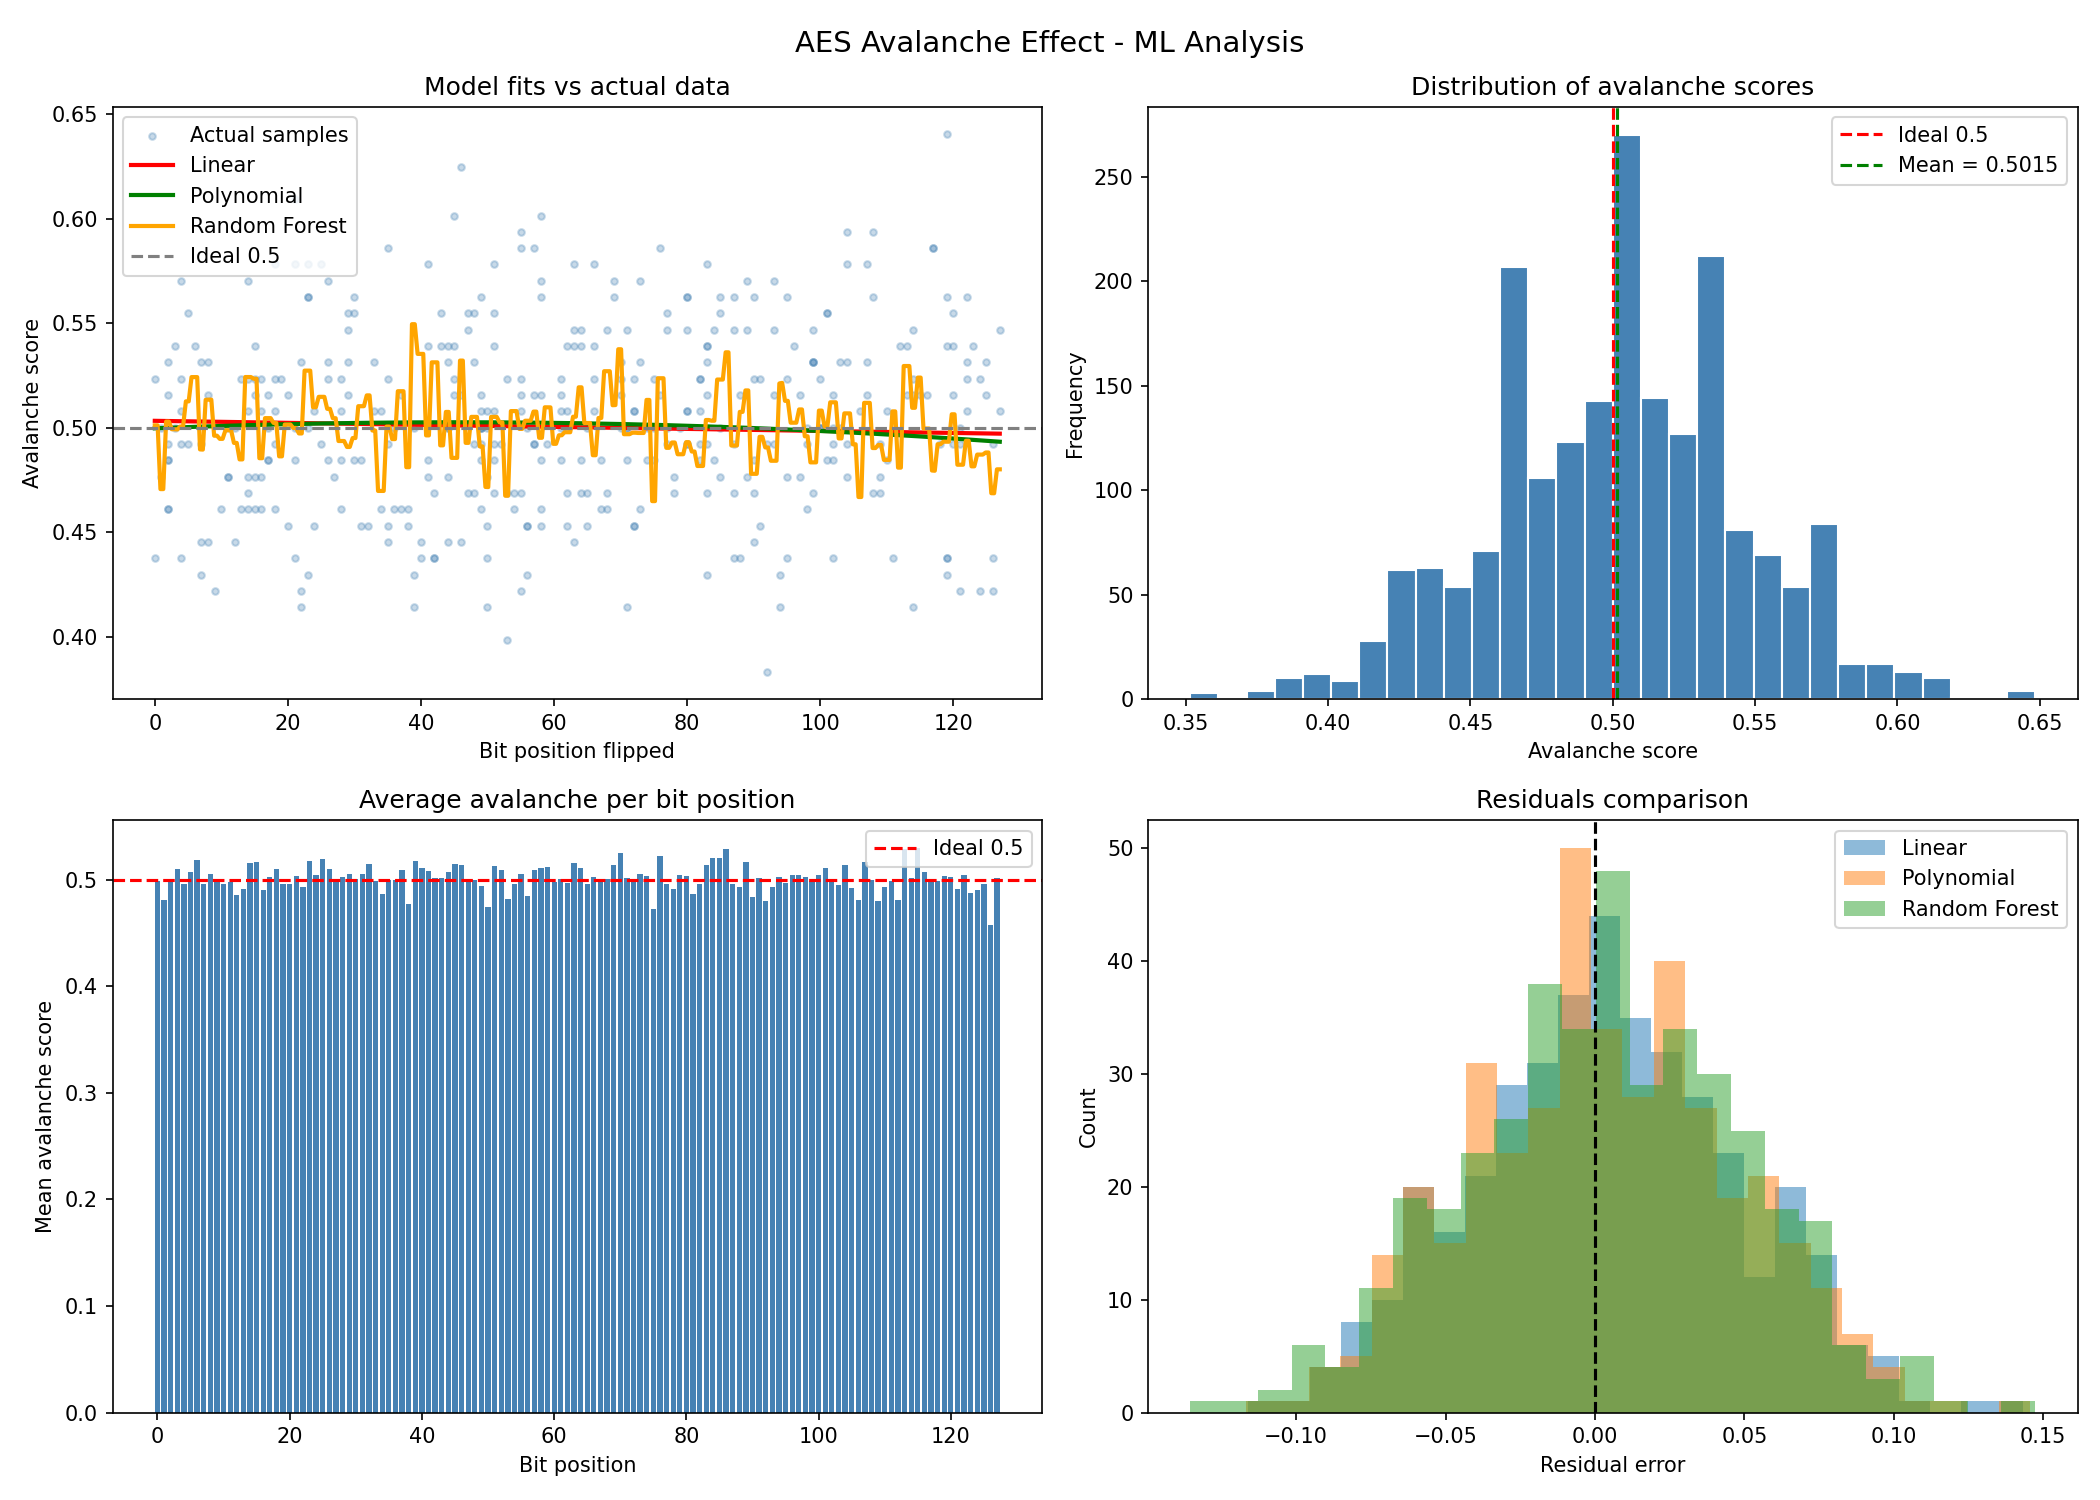
\includegraphics[width=\textwidth]{results/avalanche_analysis.png}
\caption{Machine learning analysis of AES avalanche behavior.}
\end{figure}

\section{Manual Verification}

To verify the results manually, we generated a plaintext block and flipped a single bit. After encrypting both versions, we computed the XOR difference between the ciphertexts and counted the number of changed bits.

The observed avalanche value was close to 0.5, confirming the expected diffusion property of AES.

\section{Conclusion}

Our experimental and machine learning analysis confirms that AES satisfies the avalanche property. A single-bit change in plaintext causes approximately half of the ciphertext bits to change, and the diffusion behavior is independent of the specific input bit position.

\end{document}
